\documentclass[aspectratio=169, xcolor=dvipsnames]{beamer}

\usepackage{pdfpages} % for the code of conduct
\usepackage{todonotes}
\usepackage{graphicx}
\usepackage{animate}
\usepackage{hyperref}

\usepackage[T1]{fontenc}
\usepackage{Magra}

\usepackage{tikz}
\usetikzlibrary{decorations.pathmorphing}

% \PassOptionsToPackage{dvipsnames,svgnames,x11names}{xcolor}

\hypersetup{
    colorlinks = true,
    linkbordercolor = {red}
}

% \usetheme{Madrid}
\usetheme{EastLansing}
\beamertemplatenavigationsymbolsempty

\title[Exploring Holographic QCD]{\input{title.txt}}
\author{Markus A.G. Amano}
\date{April 2nd, 2024}

\subtitle{\href{https://inspirehep.net/literature/2690368}{ arXiv:2308.11686 (Amano, Kaminski et al. 2023) }
  % \\{\tiny accepted for publication with Progress in Particle and Nuclear Physics}
}
% \institute{Yamagata University (as a JSPS Fellow)}
\institute{Yamagata University}


\begin{document}

{
  \setbeamercolor{background canvas}{bg=}
  \includepdf[pages=1]{codeofconduct.pdf}
}

\maketitle

\section{Introduction}

\begin{frame}
  \frametitle{Motivating Questions}

  \begin{columns}[c]
    \begin{column}{0.5\paperwidth}
      \begin{enumerate}
        \item What is the hydrodynamic description of QCD in the Quark Gluon Plasma phase?
        \item How does vorticity affect Quark Gluon Plasma matter?
        \item What can a holographic model tell us about nature of strongly rotating plasmas?
      \end{enumerate}
    \end{column}
    \begin{column}{0.5\paperwidth}
      \animategraphics[loop,autoplay,width=0.8\textwidth]{10}{genfigs/tensor_dance_v2-}{0}{121}
    \end{column}
  \end{columns}
\end{frame}

\subsection{Holography 101}

\begin{frame}
  \frametitle{The Holographic Description}

  \begin{block}{Holographic Principle}
    The information of the universe can be encoded on its boundaries.
  \end{block}

  \begin{block}{}
    string theory + Maldacena $\longrightarrow$ AdS/CFT
  \end{block}

  \begin{columns}[c]
    \begin{column}{0.3\paperwidth}
    \end{column}
    \begin{column}{0.4\paperwidth}
      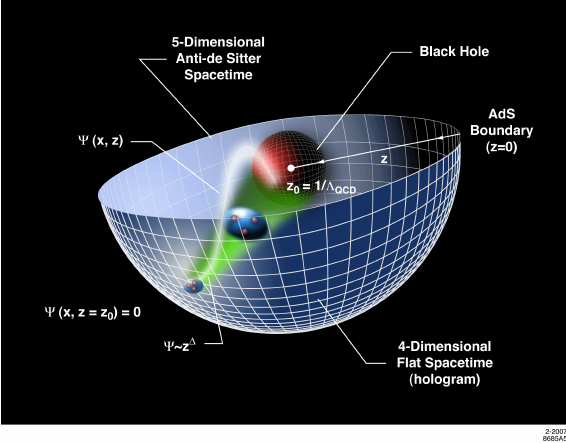
\includegraphics[height=0.3\paperwidth]{figs/AdS-CFT-The-evolution-of-the-proton-at-different-length-scales-is.png}\\
      \begin{flushright}
        {\tiny (\href{https://inspirehep.net/literature/778796}{Brodsky, Teramond 2008})}
      \end{flushright}
    \end{column}
    \begin{column}{0.3\paperwidth}
    \end{column}
  \end{columns}

\end{frame}

\begin{frame}
  \frametitle{Conformal Field Theory}
  \framesubtitle{``the field theory side''}
  % CFT
  \begin{block}{}
    \alert{CFT}(conformal field theory) is a field theory that is invariant under conformal transformations.
    $${ds}^2 \rightarrow \Omega^2 {ds}^2$$
  \end{block}

  \begin{block}{Conformal Transformations}
    \begin{itemize}
      \item Translations
      \item Rotations and Lorentz transformations
      \item \textbf{Dilations}
      \item \textbf{Special Conformal Transformations}
    \end{itemize}
  \end{block}

\end{frame}

\begin{frame}
  \frametitle{Anti de-Sitter Space}
  \framesubtitle{``the gravity side''}

  % AdS
  \begin{block}{}
    \alert{AdS}(Anti de-Sitter) is a negatively curved space that is as \textit{symmetric as} Minkowski space.
  \end{block}

  \begin{itemize}
    \item conformally flat 
      $ds^2 = \frac {\ell^2}{z^2} \left( -dt^2 + d\vec x\cdot d\vec x + dz^2 \right)$
    \item negative Curvature 
      $R = -20/\ell^2$
    \item classical gravity with matter fields
  \end{itemize}

  % \begin{equation*}
  %   S_{EH}=\frac{1}{16\pi G_5}\int d^5 x \sqrt{-g}\left(R-2\Lambda\right) +S_{ct}
  % \end{equation*}

\end{frame}

% AdS/CFT
% Action Dictionary/Witten Relation

\begin{frame}
  \frametitle{A Holographic Description}
  \framesubtitle{
    (\href{https://inspirehep.net/literature/467202}{Gubser et al 1998},
    \href{https://inspirehep.net/literature/467400}{Witten 1998}) [References \href{https://inspirehep.net/literature/1316320}{Natsuume 2012}; \href{https://www.cambridge.org/core/books/gaugegravity-duality/16CCA2E431B24AEF1B51B0F9C5BE755E}{Ammon, Erdmenger 2015}]}
  \begin{block}{GKP-Witten Relation}
    \begin{center}Z$_\text{gauge}$ = Z$_\text{AdS}$\end{center}
    % $$\left\langle \exp\left(i\int\phi^{(0)} \mathcal O_\phi\right) \right\rangle =  e^{i S_\text{on-shell}[\phi(z\rightarrow0) = \phi^{(0)}]}$$
  \end{block}

  \begin{block}{The Holographic Dictionary}
    \begin{align*}
      \text{Stress Energy Momentum Tensor}~\left\langle T_{\mu\nu}\right\rangle &\longleftrightarrow g_{\mu\nu}\\
      \text{Charge Current}~\left\langle J_{\mu}\right\rangle &\longleftrightarrow A_{\mu}
      % \left\langle\mathcal O_\phi\right\rangle &\longleftrightarrow \phi
    \end{align*}
  \end{block}

  % put a column in the bottom if possible

\end{frame}

\subsection{Making a Dual State}

\begin{frame}
  \frametitle{Adding Temperature}

  \begin{block}{}Non-zero Temperature $\longleftrightarrow$ Event Horizon\end{block}

  $$\frac {\ell^2}{z^2} \left( -dt^2 + d\vec x\cdot d\vec x + dz^2 \right) \rightarrow \frac {\ell^2}{z^2} \left( -f(z) dt^2 + d\vec x\cdot d\vec x + \frac 1{f(z)}dz^2 \right)$$
  % \begin{block}{}
  %   % $$ f(z) = 1 - z^3/z_h^2 $$
  % \end{block}

  \begin{center}
    \scalebox{0.9}{
      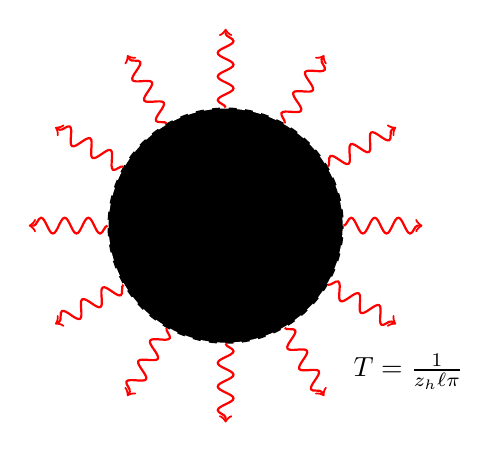
\begin{tikzpicture}
        % Draw a black hole
        \fill[black] (0,0) circle (1.5cm);

        % Draw the event horizon
        \draw[dashed, white, thick] (0,0) circle (1.5cm);

        % Draw squiggly arrows representing Hawking radiation
        \foreach \i in {0,30,...,330}
        {
          \draw[->, red, thick, decorate, decoration={snake, amplitude=1mm, segment length=3mm}] (\i:1.5cm) -- (\i:2.5cm);
        }

        % Add the equation for Hawking temperature
        \node[below right] at (1.5,-1.5) {$T=\frac{1}{z_h\ell\pi}$};
      \end{tikzpicture}
    }
  \end{center}
\end{frame}

\begin{frame}
  \frametitle{Adding Rotation}
  \framesubtitle{at non-zero temperature}

  \begin{block}{}rotation $\longleftrightarrow$ event horizon that rotates relative to the boundary\end{block}

  \begin{block}{}
    $\frac {\ell^2}{z^2} \left( -f(z) dt^2 + d\vec x\cdot d\vec x + \frac 1{f(z)}dz^2 \right) \rightarrow$ \\$(4+1)$D Myers-Perry AdS Black Hole (\href{https://inspirehep.net/literature/478927}{Hawking et al 1998})
  \end{block}

  \begin{alertblock}{global AdS vs local patch}
    \begin{itemize}
      \item Global AdS $\leftrightarrow$ spherical boundary\\
      \item Local patch (zoomed in version of Global AdS) $\leftrightarrow$ planar boundary
    \end{itemize}
  \end{alertblock}

  % \missingfigure{Zooming into a rotating black hole image to show relation between local and global views.}

\end{frame}

% Angular momentum (and angular velocity)
% 5d two angular momentum, 4d one angular momentum

\begin{frame}[squeeze]
  \frametitle{Mapping 4D Rotation to 3D}
  \begin{itemize}
    \item Two independent planes of rotation in $4$D 
    \item Hopf Coordinates: 
      \begin{align*}
        &x=\cos\psi_H\sin \theta_H\,,&y=\sin \psi_H\sin \theta_H\\
        &z=\cos \phi_H\cos \theta_H\,,&w=\sin \phi_H\cos \theta_H
      \end{align*}
    \item Angular Momentum Vector $J = a\frac\partial{\partial\psi_H} + b\frac\partial{\partial\phi_H}$
  \end{itemize}
  \begin{columns}[c]
    \begin{column}{0.5\paperwidth}
      \href{https://markuspad.com/figures/axis_lines.html}{\includegraphics[height=0.5\paperheight]{genfigs/axis_lines.pdf}}
    \end{column}
    \begin{column}{0.5\paperwidth}
      \href{https://markuspad.com/figures/hopf_links.html}{\includegraphics[height=0.5\paperheight]{genfigs/hopf_links.pdf}}
    \end{column}
  \end{columns}
  % Interactive Versions here and here
\end{frame}

\section{Our Research}

% \begin{frame}
%   \frametitle{Our Research Goals}
%   \framesubtitle{and what we did}
%   \missingfigure{Add the goals}
% \end{frame}

% \begin{frame}
%   \frametitle{Our Research Goals}

%   \begin{itemize}
%     \item Non-hydrodynamic quasinormal mode spectrum of equal angular momentum AdS black hole
%     \item Emergence of fluid dynamics at large angular momenta
%     \item Strongly coupled quantum fluid hydrodynamic dispersion relations
%     \item Strongly coupled quantum fluid thermodynamic equation of state
%   \end{itemize}

% \end{frame}

\subsection{The Rotating Geometry}

% Simplifying Angular Momentum Configuration and the axis-full Configuration
\begin{frame}[squeeze]
  \frametitle{Equal Angular Momentum Black Hole}
  \framesubtitle{A ``Simply Spinning'' Black Hole}

  \begin{block}{Enhanced Symmetry}
    There is enhanced the symmetry with $a=b$.
    \begin{center}$U(1)\times U(1) \longrightarrow SU(2)\times U(1)$ \end{center}
  \end{block}

  \begin{equation*}
    \begin{aligned}
      % d s^2=\frac 1{G(r)}{dr}^2-\left(\frac{r^2}{\ell^2}+1\right)dt^2&+\frac 14 r^2 \left((\sigma^1)^2+(\sigma^2)^2+(\sigma^3)^2\right) \\ &+\frac{2 \mu  }{r^2} \left(\frac a2 \sigma^3+dt\right)^2
      d s^2=\frac 1{G(r)}{dr}^2-\left(\frac{r^2}{\ell^2}+1\right)dt^2&+\frac 14 r^2 \left(\sigma^+ \sigma^- +\sigma^- \sigma^+ +(\sigma^3)^2\right) \\ &+\frac{2 \mu  }{r^2} \left(\frac a2 \sigma^3+dt\right)^2
    \end{aligned}
  \end{equation*}

  \begin{itemize}
    \item Coordinates: $(t, \theta, \phi, \psi, r)$
    \item $\sigma$'s for the metric of a 3D sphere
    \item $r_+ \equiv$ outer horizon, $\left(G(r_+)=0\right)$
    \item Angular momentum Vector $a\frac\partial{\partial\psi} \leftrightsquigarrow \sigma^3$ 
  \end{itemize}

\end{frame}

\subsection{Metric Perturbations}

\begin{frame}
  \frametitle{Perturbing Field Theory}
  \framesubtitle{with metric perturbations [\href{https://inspirehep.net/literature/209356}{Reference Wald 1984 pg. 183}]}

  \begin{block}{Perturbed Metric}
    \begin{equation*}
      g^{p}_{\mu\nu} {dx}^\mu {dx}^\nu = \left(g_{\mu\nu}+\epsilon~h_{\mu\nu}+O(\epsilon^2)\right) {dx}^\mu {dx}^\nu
    \end{equation*}

    \begin{equation*}
      \left\langle \delta T_{\mu\nu}\right\rangle\longleftrightarrow h_{\mu\nu}
    \end{equation*}
  \end{block}

  \begin{block}{Einstein Field Equations at First Order}
    \begin{equation*}
      -\frac{1}{2}\nabla_\mu \nabla_\nu h-\frac{1}{2}\nabla^\lambda \nabla_\lambda h_{\mu\nu}+\nabla^\lambda \nabla_{(\mu}h_{\nu)\lambda} = \textcolor{red}{\frac{2\Lambda}{D-2}h_{\mu\nu}}
    \end{equation*}
  \end{block}

  % The Einstein Field Equations at first order ([Wald 1984][wald1984]) are linear PDEs.

  \begin{block}{Enhanced Symmetry}
    \begin{center}PDEs $\rightarrow$ Decoupled set of ODEs\end{center}
  \end{block}

\end{frame}

\begin{frame}
  \frametitle{Perturbation Metric Decomposition}

  \begin{align*}
    h_{\mu\nu} = \int d\omega e^{-i\omega t} \sum_{\mathcal{J}, \mathcal{K}', \mathcal{M},i,j} h_{i j}(r;\omega,\mathcal{J},\mathcal{M},\mathcal{K}') \sigma^i_{\mu} \sigma^j_{\nu} D_{\mathcal{K'}-Q(\sigma^{i})-Q(\sigma^{j}) \mathcal{M}}^\mathcal{J}
  \end{align*}

  \begin{itemize}
    \item $\mathcal{J} > 0$, $-\left( \mathcal J + 2 \right) \leq \mathcal{K}' \leq \mathcal J + 2$, $-\mathcal J \leq \mathcal{M}'  \leq \mathcal J$
    \item $i, j \in \{t,r,3,+, -\}$
    \item $\sigma^t := dt$ and $\sigma^r := dr$
  \end{itemize}

  \begin{block}{Axial Angular Momentum Eigenfunction}
    \alert{$Q$} is the angular momentum quantum charge of $\sigma^i$ and eigenfunction of $W_3 := i\partial_\psi$

    \begin{equation*}
      Q(\sigma^i) = 0 \text{ if } i=r,t,3;\quad 1 \text{ if } i=+;\quad -1 \text{ if } i=- 
    \end{equation*}
  \end{block}

\end{frame}

\begin{frame}
  \frametitle{Decomposition Facts}
  \framesubtitle{plugging the decomposed perturbation in to its equations of motion}

  \begin{itemize}
    \item $((\mathcal J, \mathcal M), \mathcal K')$ perturbations decouple
    \item $\mathcal M$ vanishes from equations
  \end{itemize}

  \vfill

  \begin{description}
    \item[Tensor]
      \(\mathcal K' = \mathcal J + 2\); \(h_{++}\)
    \item[Vector]
      \(\mathcal K' = \mathcal J + 1\); \(h_{+r}\), \(h_{+t}\), \(h_{+3}\) (,
      and \(h_{++}\) if \(\mathcal J \geq 1\))
    \item[Scalar]
      \(\mathcal K' = \mathcal J\), \(h_{+-}\); \(h_{ab}\) where
      \(a,b \in \{r,t,3\}\)\\
      (, \(h_{+r}\), \(h_{+t}\), \(h_{+3}\) if \(\mathcal J \geq 1\) ) (, and
      \(h_{++}\) if \(\mathcal J \geq 2\))
  \end{description}
\end{frame}

% Hydrodynamics
% Hydroydnamics Expansion
% Critical Point (Maybe)

\subsection{Hydrodynamics}

\begin{frame}{Quasinormal Modes and Hydrodynamic Expansion}

  \begin{equation*}
    h_{\mu\nu} \sim r^2 h^{(0)}_{\mu\nu} - h^{(1)}_{\mu\nu}/r^2
  \end{equation*}

  \begin{itemize}
    \item \(h^{(0)}_{\mu\nu}\) \(\leftrightarrow\) source of
      \(\delta T\).
    \item \(h^{(1)}_{\mu\nu}\) \(\leftrightarrow\) VEV of
      \(\delta T_{\mu\nu} \equiv \langle \delta T_{\mu\nu} \rangle\).
  \end{itemize}

  \vfill


  \begin{block}{Quasinormal Modes (QNMs)}
    QNMs are $h$ and frequencies, $\omega$, that satisfy
    \begin{itemize}
      \item Equations of motion
      \item \(h^{(0)}_{\mu\nu} = 0\), sourceless boundary condition
      \item Ingoing Boundary Condition at the horizon
    \end{itemize}
  \end{block}

  \vfill

  \begin{itemize}
    \item \textbf{ Hydrodynamic Expansion } $\omega = \sum_{i=0} \omega_{(i)} k^i$
  \end{itemize}

  % \begin{block}{}
  % \end{block}

\end{frame}

% Near Boundary Expansion
% Source/VEV
% Sourcless Perturbations -> Non-Hermitian Operator -> Quasinormal Modes -> Dual Spectrum
% Hydrodynamics
% Hydroydnamics Expansion
% Critical Point (Maybe)

\section{Results}

\begin{frame}{Results}

  (\href{https://arxiv.org/abs/2308.11686}{Amano, Kaminski et al. 2023})

  \begin{itemize}
    \item Non-Hydrodynamic Modes and the effects of non-extremal rotation.
      \begin{itemize}
        \item Tensor
        \item Vector
        \item Scalar
      \end{itemize}
    \item Cross Spectrum Comparison
    \item The Emergence of Hydrodynamics
      % \item Stability
    \item Large Temperature Hydrodynamic Transport
  \end{itemize}
\end{frame}

\subsection{Non-hydrodynamic Modes}

\begin{frame}{\(\mathcal K' = \mathcal J + 2\) Tensor Sector}
  \begin{center}
      \animategraphics[loop,autoplay,width=0.5\textwidth]{10}{genfigs/tensor_dance_v2-}{0}{121}
  \end{center}

  \(\mathcal K' = \mathcal J + 2\); \(h_{++}\)
\end{frame}

\begin{frame}{\(\mathcal K' = \mathcal J + 1\) Vector Fluctuations}
  \begin{columns}[T]
    \begin{column}{0.33\textwidth}
      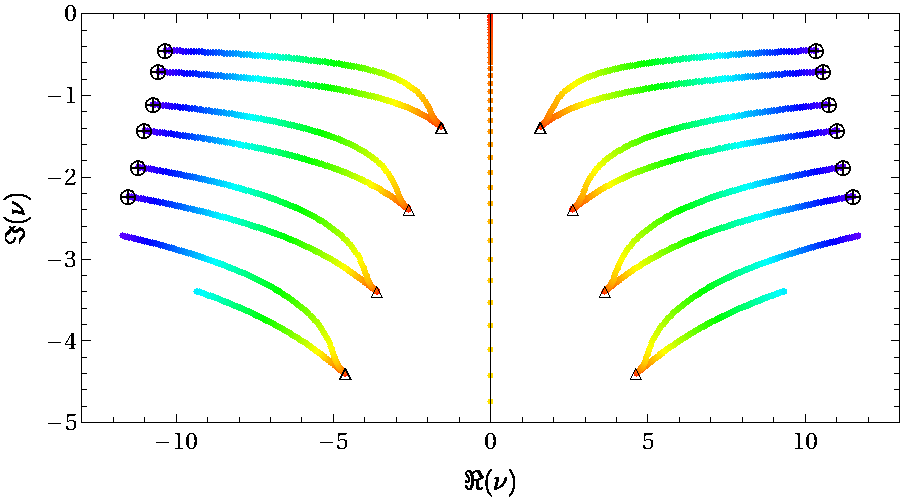
\includegraphics[width=1.05\textwidth]{figs/Vector_rp_10_grid_45_a_0.pdf}
    \end{column}

    \begin{column}{0.33\textwidth}
      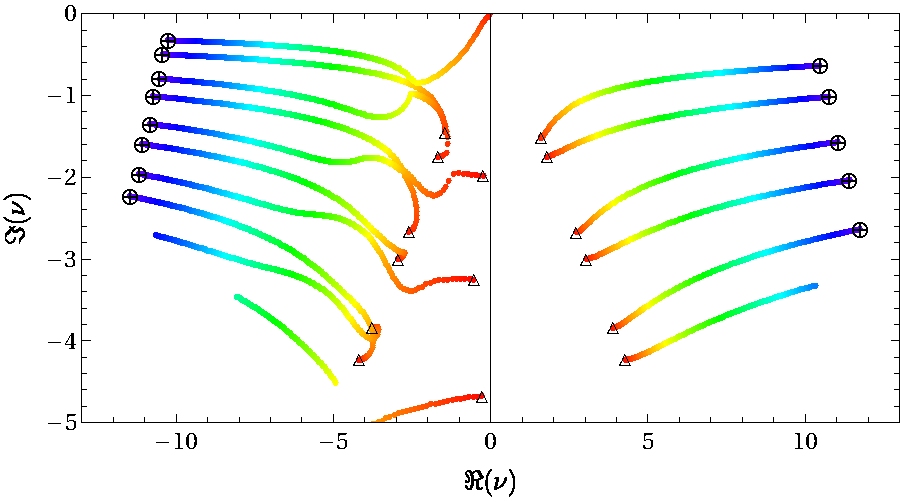
\includegraphics[width=1.05\textwidth]{figs/Vector_rp_10_grid_45_a_1_2.pdf}
    \end{column}

    \begin{column}{0.33\textwidth}
      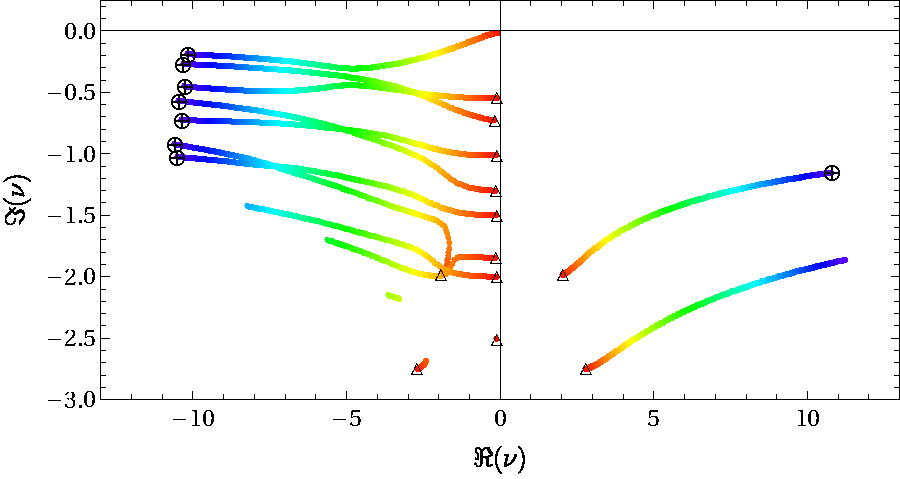
\includegraphics[width=1.05\textwidth]{figs/Vector_rp_10_grid_45_a_9_10.pdf}
    \end{column}
  \end{columns}

  \vfill

  \begin{columns}[c]
    \begin{column}{0.5\textwidth}
      \(a/\ell \in \{0, 1/2, 9/10\}\)\\
      \(\mathcal K' = \mathcal J + 1\); \(h_{+r}\), \(h_{+t}\), \(h_{+3}\) 
      (and \(h_{++}\) if \(\mathcal J \geq 1\))
    \end{column}

    \begin{column}{0.5\textwidth}
      \(\mathcal J = 0, 1/2, 1, \ldots, 199/2, 100\), \(r_+/\ell = 10\)\\
      \(\bigtriangleup \equiv \mathcal J = 0\),
      \(\bigoplus \equiv \mathcal J = 100\)
    \end{column}
  \end{columns}
\end{frame}

\begin{frame}{\(\mathcal K' = \mathcal J\) Scalar Fluctuations}

  \begin{columns}[T]
    \begin{column}{0.33\textwidth}
      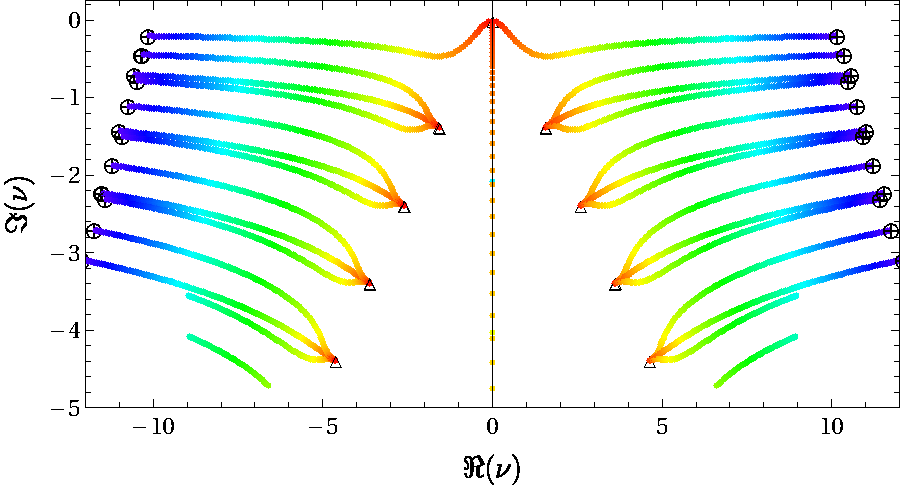
\includegraphics[width=1.05\textwidth]{figs/scalar_ef_spherical_a0.pdf}
    \end{column}

    \begin{column}{0.33\textwidth}
      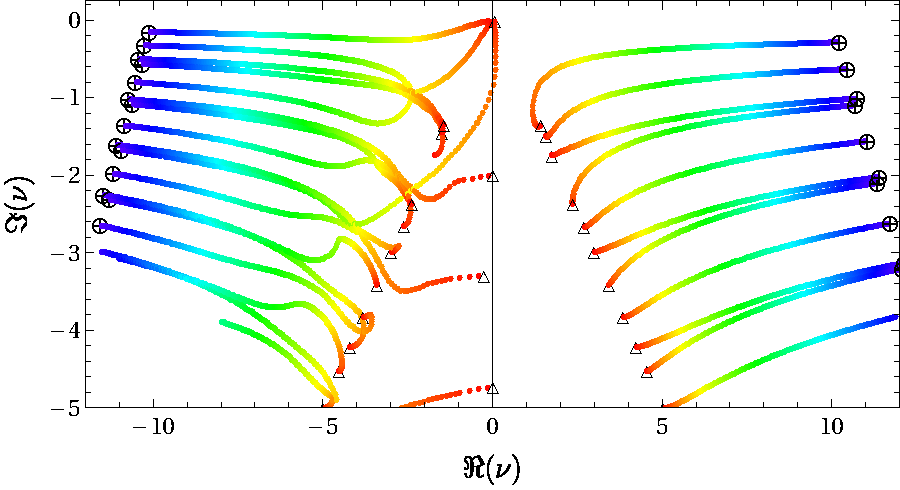
\includegraphics[width=1.05\textwidth]{figs/scalar_ef_spherical_a1_2.pdf}
    \end{column}

    \begin{column}{0.33\textwidth}
      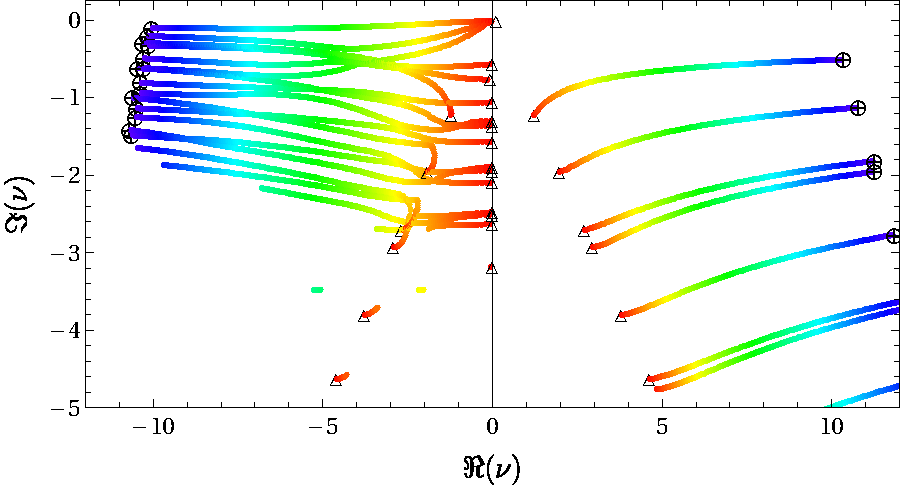
\includegraphics[width=1.05\textwidth]{figs/scalar_ef_spherical_a9_10.pdf}
    \end{column}
  \end{columns}

  \vfill

  \begin{columns}[c]
    \begin{column}{0.5\textwidth}
      \(a/\ell \in \{0, 1/2, 9/10\}\)\\
      \(\mathcal K' = \mathcal J\), 
      \(h_{+-}\) \\ \(h_{ab}\) where
      \(a,b \in \{r,t,3\}\)\\
      (, \(h_{+r}\), \(h_{+t}\), \(h_{+3}\) if \(\mathcal J \geq 1\) ) (, and
      \(h_{++}\) if \(\mathcal J \geq 2\))
    \end{column}

    \begin{column}{0.5\textwidth}
      \(\mathcal J = 0, 1/2, 1, \ldots, 199/2, 100\), \(r_+/\ell = 10\)\\
      \(\bigtriangleup \equiv \mathcal J = 0\),
      \(\bigoplus \equiv \mathcal J = 100\)
    \end{column}
  \end{columns}
\end{frame}

\begin{frame}{Cross Spectrum Comparisons}
  \begin{columns}[T]
    \begin{column}{0.5\textwidth}
      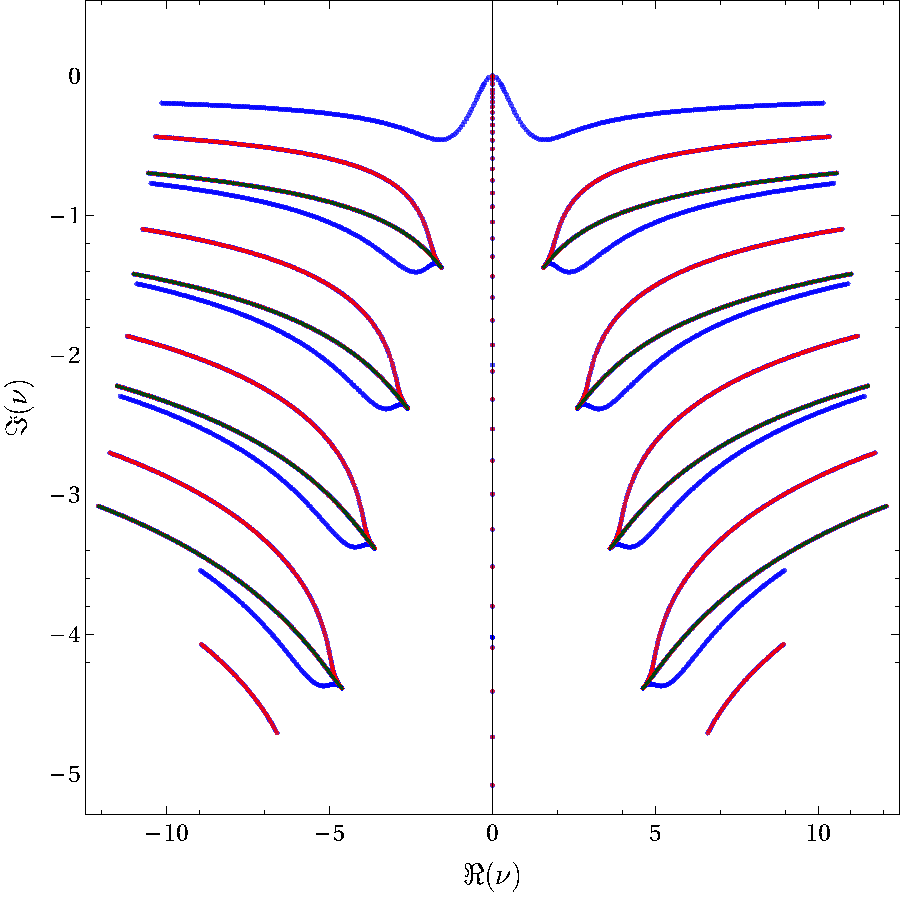
\includegraphics[width=0.8\textwidth]{figs/all_sectors_compared_ef_spherical_over_a0.pdf}
    \end{column}

    \begin{column}{0.5\textwidth}
      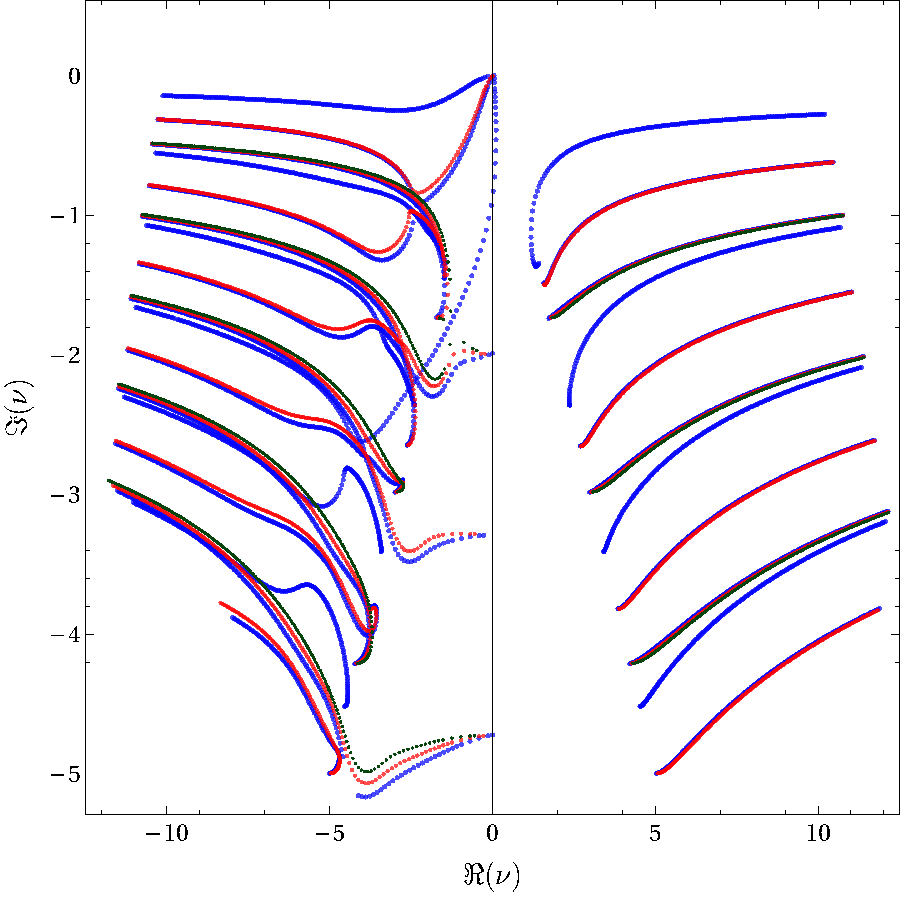
\includegraphics[width=0.8\textwidth]{figs/all_sectors_compared_ef_spherical_over_a1_2.pdf}
    \end{column}
  \end{columns}

  \vfill

  \begin{columns}[c]
    \begin{column}{0.33\textwidth}
      \textcolor{ForestGreen}{$\cdot$ Tensor}
    \end{column}

    \begin{column}{0.33\textwidth}
      \textcolor{red}{$\cdot$ Vector}
    \end{column}

    \begin{column}{0.33\textwidth}
      \textcolor{blue}{$\cdot$ Scalar}
    \end{column}
  \end{columns}
\end{frame}

\subsection{The Emergence of Hydrodynamics}

\begin{frame}{The Emergence of Hydrodynamics}
  To study the dispersion relations of the lowest gapless modes, we looked
  at the momentum diffusion sector.

  \vfill

  We solved spectra for
  \(r_+ = \{10, 100, 1000, 10^4 , 10^5 , 10^6 , 10^7 \}\) and
  \(\mathcal J = 0, 1/2, 1, \ldots, \mathcal J_\mathrm{max}\).

  \begin{alertblock}{}
    {\(\mathcal J_\mathrm{max}/r_+ = \mathit j_\mathrm{max} = 0.1\)}
  \end{alertblock}

  \vfill

  To see the emergence of hydrodynamics, we fitted the data to the
  equation below with fitting parameters \(\alpha\), \(\beta\), \(D\), and
  \(v\).

  \vfill

  \begin{equation*}
    \omega = v \mathcal J^\beta - i D \mathcal J^\alpha
  \end{equation*}
\end{frame}

\begin{frame}
  \begin{columns}[c]
    \begin{column}{0.5\textwidth}
      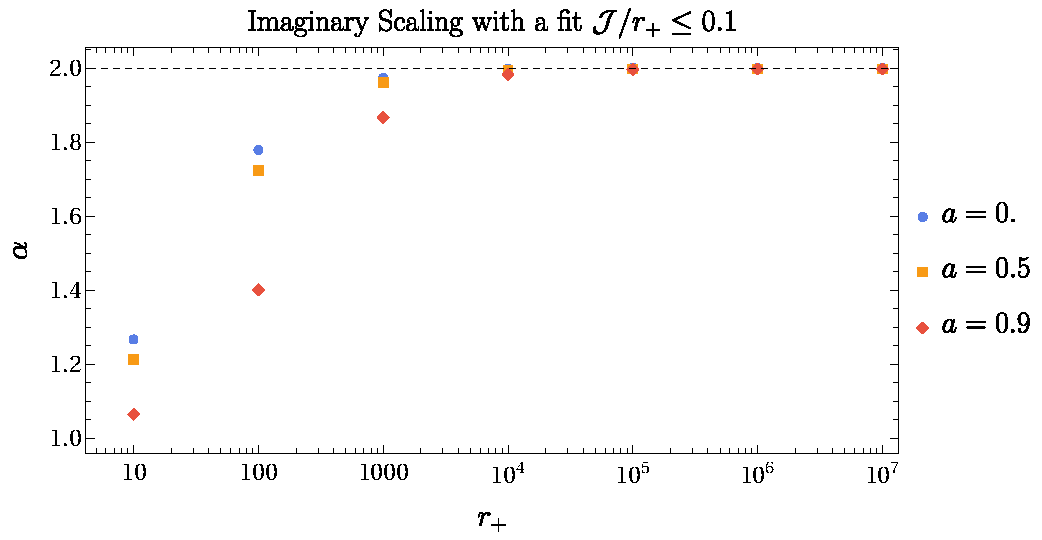
\includegraphics[width=0.9\textwidth]{figs/vector_dispersive_mode_rp_vs_im_scaling_over_a_scaled_Jleq0_1.pdf}\\
      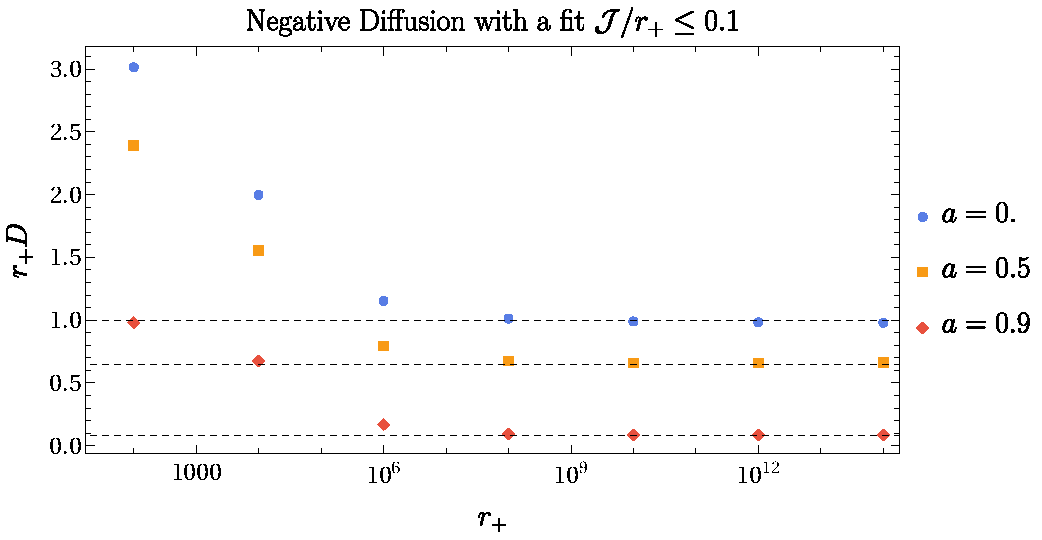
\includegraphics[width=0.9\textwidth]{figs/vector_dispersive_mode_rp_vs_diffusion_over_a_scaled_Jleq0_1.pdf}
    \end{column}

    \begin{column}{0.5\textwidth}
      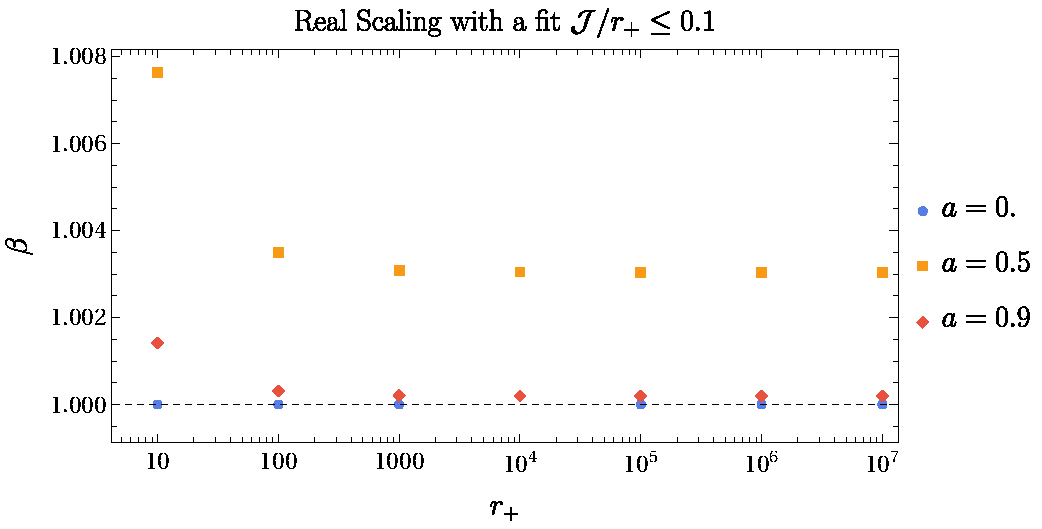
\includegraphics[width=0.9\textwidth]{figs/vector_dispersive_mode_rp_vs_re_scaling_over_a_scaled_Jleq0_1.pdf}\\
      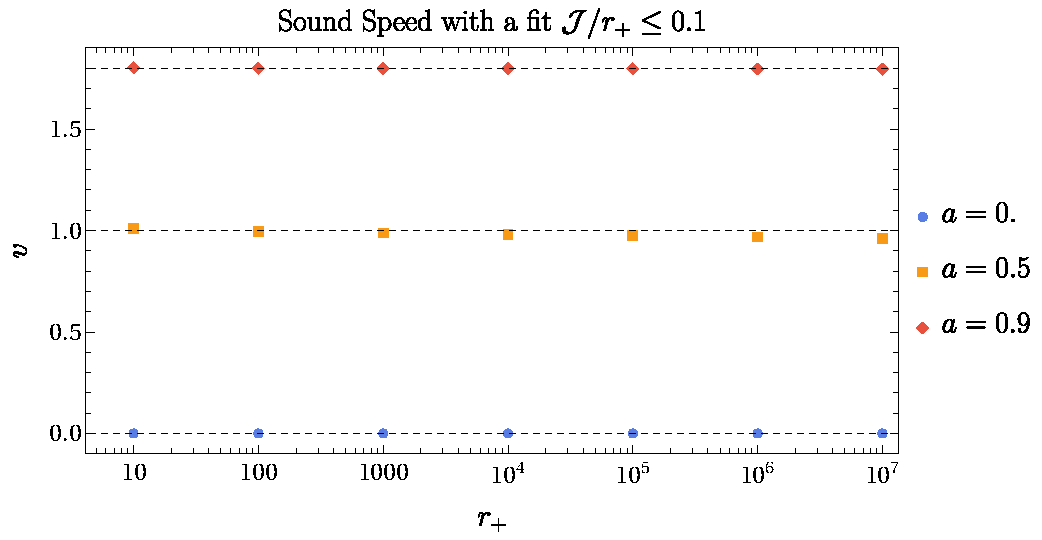
\includegraphics[width=0.9\textwidth]{figs/vector_dispersive_mode_rp_vs_soundspeed_over_a_scaled_Jleq0_1.pdf}
    \end{column}
  \end{columns}

  \vfill

  \begin{columns}[c]
    \begin{column}{0.5\textwidth}
      Relativistic Dispersion Relation (\href{https://inspirehep.net/literature/1744607}{Kovtun 2019})
    \end{column}

    \begin{column}{0.5\textwidth}
      \begin{equation*}
        \omega = v \mathcal J^\beta - i D \mathcal J^\alpha
      \end{equation*}
    \end{column}
  \end{columns}
\end{frame}

\subsection{Large Temperature Limit}

\begin{frame}[squeeze]
  \frametitle{Large Temperature Limit}
  \framesubtitle{(\href{https://inspirehep.net/literature/1806001}{Garbiso, Kaminski 2020})}

  \begin{itemize}
    \item $r_+ \to \infty$ in QNM fluctuation equations
    \item Spinning black hole geometry dual to a boosted fluid
    \item Dual field theory on small patch of $S^3 \approx \mathbb{R}^3$
  \end{itemize}

  \begin{block}{Rescaling}
    \begin{equation*}
      \begin{aligned}
        \omega &\to \alpha 2\nu r_+/\ell \\
        \mathcal{J} &\to \alpha j r_+/\ell \\
        r_+ &\to \alpha r_+ \\
        r &\to \alpha r\\
        \quad \alpha&\to\infty
      \end{aligned}
    \end{equation*}
  \end{block}

  \begin{alertblock}{}
    Leading order terms in $\alpha$ kept
  \end{alertblock}

\end{frame}

\begin{frame}
  \frametitle{Equation of State}

  \begin{block}{Thermodynamic Relation}
    \begin{center}
      $\epsilon + \Phi_5 = s \, T + 2\mathfrak{j}\Omega$
    \end{center}
  \end{block}

  {\small
    \begin{eqnarray*}
      s&\sim& \frac{r_+^3}{4 G_5 \ell^2 \sqrt{\ell^2-a^2}} \\
      \epsilon &\sim& \frac{\mu (a^2+3 \ell^2)}{8 \pi G_5 \ell^4} \\ 
      P_\perp &\sim& \frac{\mu (\ell^2-a^2) }{8 \pi G_5 \ell^4}\, , \quad P_{||} \sim \frac{\mu (3 a^2+ \ell^2)}{8 \pi G_5 \ell^4} \\
      \mathfrak{j} &\sim& \frac{a \mu}{2\pi \ell^2 G_5}  \, , \quad \Omega \sim \frac{a}{\ell^2}\\ 
      \mu &\sim& \frac{r_+^4}{2 (\ell^2 - a^2)} \,,\quad T \sim \frac{\sqrt{\ell^2-a^2}~r_+}{\pi \ell^3}
    \end{eqnarray*}
  }

\end{frame}

\begin{frame}[squeeze]
  \frametitle{Large Temperature Hydrodynamic Transport}
  \framesubtitle{Shear Sector}
  \begin{figure}
    \centering
    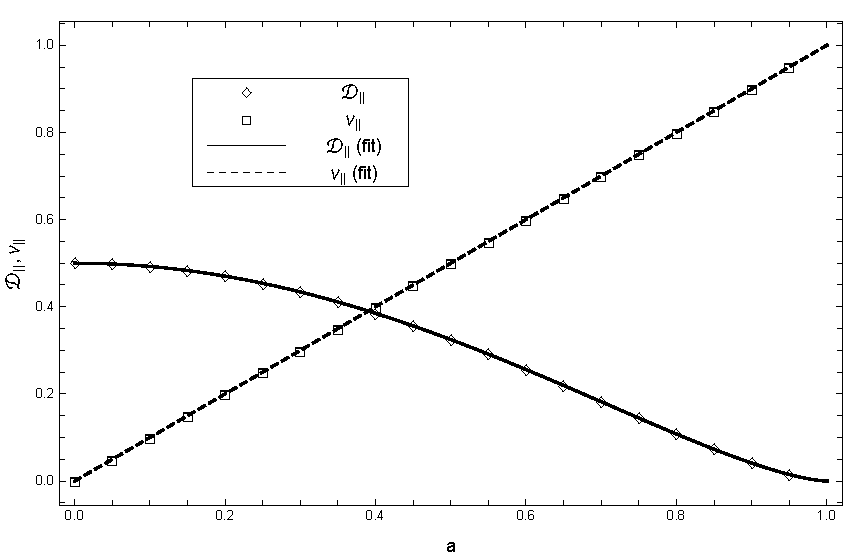
\includegraphics[width=0.5\paperwidth]{figs/htp_h3p_rinf_hydro_DiffusionPropagationOverA.pdf}
  \end{figure}

  \begin{columns}[c]
    \begin{column}{0.4\textwidth}
      \(h_{+r}\), \(h_{+t}\), \(h_{+3}\)\\
      Relativistic Dispersion Relation (\href{https://inspirehep.net/literature/1744607}{Kovtun 2019})
    \end{column}

    \begin{column}{0.4\textwidth}
      \begin{equation*}
        \nu = a j - i \frac 12 (1-a^2)^{3/2} j^2
      \end{equation*}
    \end{column}
  \end{columns}

\end{frame}

\begin{frame}
  \frametitle{Large Temperature Hydrodynamic Transport}
  \framesubtitle{Sound Sector}
  \begin{figure}
    \centering
    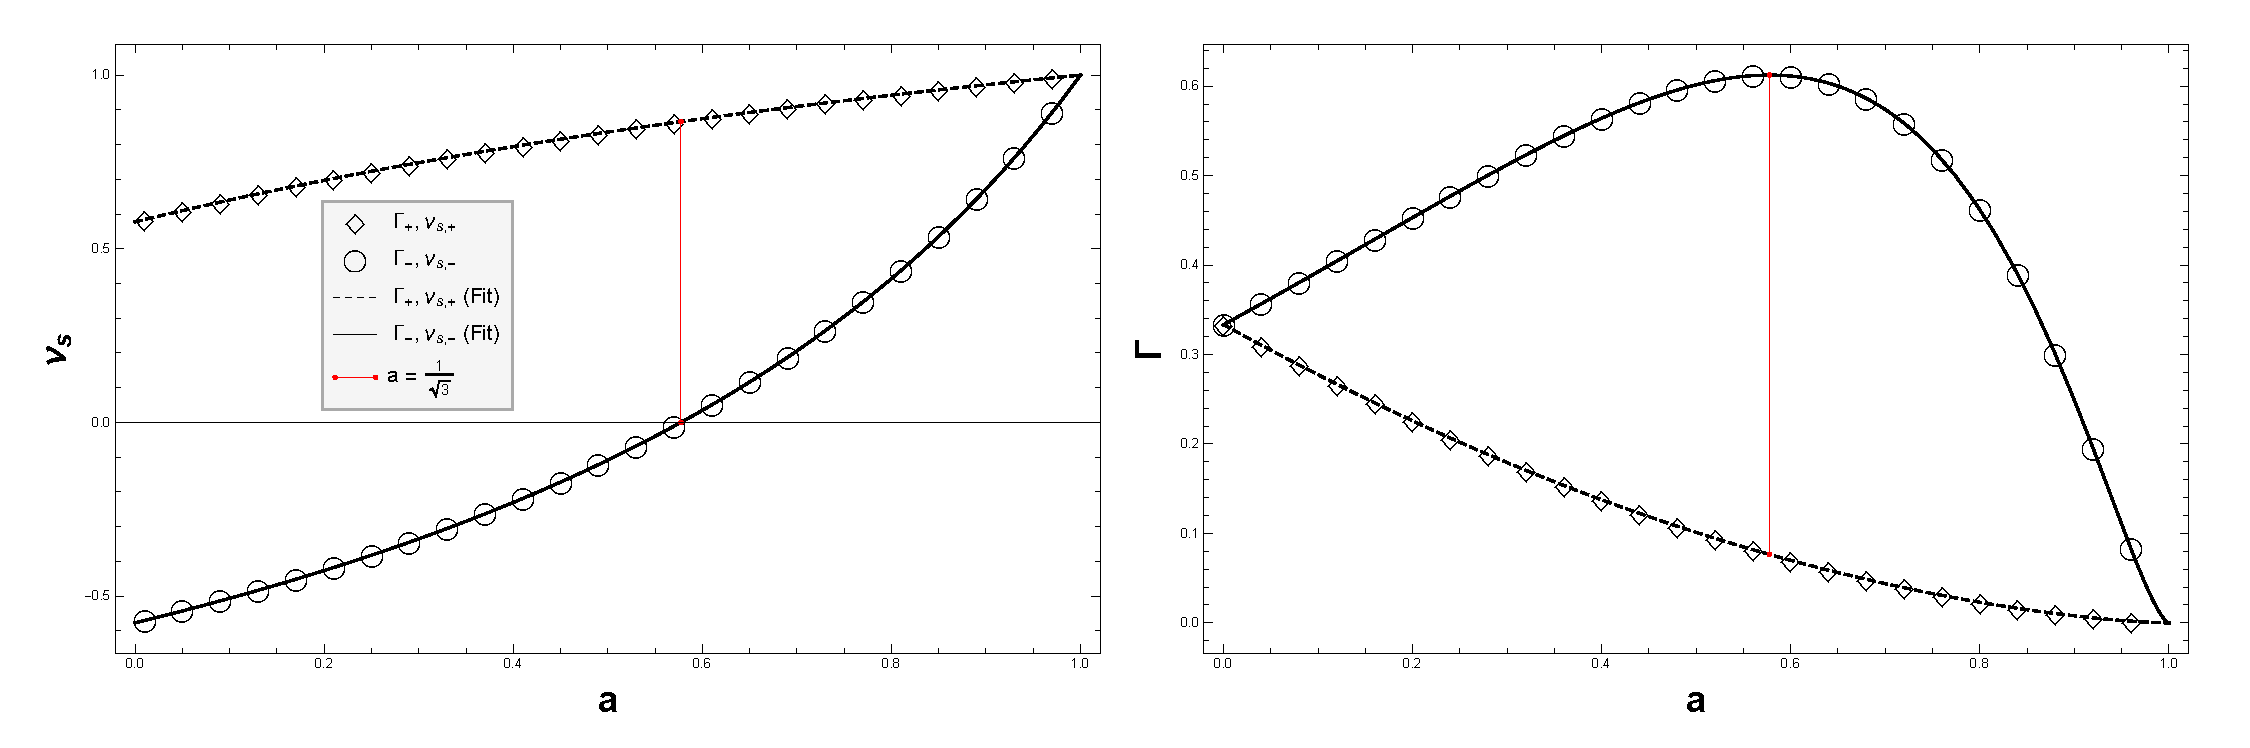
\includegraphics[width=0.9\paperwidth]{figs/scalar_rinf_hydro_DiffandPropOverA.pdf}
  \end{figure}

  \begin{columns}[c]
    \begin{column}{0.4\textwidth}
      \(h_{+-}\), \(h_{ab}\) where \(a,b \in \{r,t,3\}\)\\
      Relativistic Dispersion Relation (\href{https://inspirehep.net/literature/1744607}{Kovtun 2019})
    \end{column}

    \begin{column}{0.4\textwidth}
      \begin{equation*}
        \nu = \frac{v_0\pm v_s}{1\pm v_0 v_s} j - \frac{i}{2} {\Gamma_0} \frac{(1-v_0^2)^{3/2}}{(1\pm v_0 v_s)^3} j^2
      \end{equation*}
    \end{column}
  \end{columns}

\end{frame}  

\section{Conclusion}

\begin{frame}{Summary and Outlook}

  \begin{block}{Outlook}
    \begin{itemize}
      \item
        Look to calculate with a more general parameter space where
        \(\mathcal J_\phi\neq\mathcal J_\psi\) (\(a\neq b\)).

        \begin{itemize}
          \item
            No ``axis of rotation'' in current background.
          \item
            Need to solve 2 Variable PDE (\href{https://inspirehep.net/literature/1780844}{Amado et
            al 2020}, \href{https://inspirehep.net/literature/1844790}{Amado et
            al.~2021})
        \end{itemize}
      \item
        Different \textbf{sources} of rotation?

        \begin{itemize}
          \item
            Vector graviton sourcing the rotation $\sim$ 
            \(H_{\theta i} \sim \Omega_i r^2\)
          \item
            RN with magnetic field, \(A_\theta \sim \Omega_i r^2\)
            (\href{https://inspirehep.net/literature/854786}{Domenech et al.~2010})
        \end{itemize}
      \item
        Interpretation of linear instability in the dual field theory?
      \item Implementation in hydrodynamic models
      \item
        Expand on the dynamics of $SU(2)\times U(1)$
    \end{itemize}
  \end{block}

\end{frame}

\begin{frame}{Acknowledgements}

  This research was conducted with funding from the \emph{Postdoctoral
  Fellowship at Henan University}.

  \vfill 

  I would like to thank my collaborators, \emph{Matthias Kaminski}, \emph{Casey
  Cartwright}, and \emph{Jackson Wu}, on yet another fruitful collaboration for
  the research presented in this presentation.

  \vfill 

  Research in this presentation also included contributions from

  \begin{block}{Contributions}
    {\small
    \begin{itemize}
      \item
        \emph{Mike Blake}, \emph{Casey Cartwright}, \emph{Matthias Kaminski},
        and \emph{Anthony Thompson}\\
        (\href{https://inspirehep.net/literature/2174613}{Amano et al.~2022})
      \item
        \emph{Casey Cartwright}, \emph{Matthias Kaminski}, \emph{Jorge
        Noronha}, \emph{Enrico Speranza}\\
        (\href{https://inspirehep.net/literature/1994753}{Cartwright et al.~2023})
    \end{itemize}
  }
  \end{block}

\end{frame}

% Explain Tree

% CFT
% AdS
% AdS/CFT
% Action Dictionary/Witten Relation
% AdS Black Hole
% Temperature
% AdS MP AdS Black Hole
% Angular momentum (and angular velocity)
% 5d two angular momentum, 4d one angular momentum
% Simplifying Angular Momentum Configuration and the axis-full Configuration
% Linear Perturbations
% Near Boundary Expansion
% Source/VEV
% Sourcless Perturbations -> Non-Hermitian Operator -> Quasinormal Modes -> Dual Spectrum
% Hydrodynamics
% Hydroydnamics Expansion
% Critical Point (Maybe)

% Research Motivations
% rotating fluids are ubiquitous 
% Heavy-Ion Collisions at RHIC possess large vorticity
% The holography offers a microscopic to derive an equation of state
% Rotating black holes in holography are dual an equilibrated rotating fluid
% Perturbing the geometry is equivalent to perturbing the fluid allowing for hydrodynamic description the said fluid

\end{document}
